\documentclass{acm_proc_article-sp}

\begin{document}

\title{Vesicle-Synapsin Interactions Modeled with Cell-DEVS}

\numberofauthors{1}

\author{ \alignauthor Rhys Goldstein \\ 
    \affaddr{Department of Systems and Computer Engineering}\\
    \affaddr{Carleton University}\\
    \affaddr{Ottawa, Ontario, Canada}\\
    \email{rhys@sce.carleton.ca} }

\maketitle

\keywords{DEVS formalism, cellular automata, presynaptic nerve terminal, vesicle, synapsin}

\section{Introduction}
The interactions of vesicles and synapsins were 
modeled using the Cell-DEVS formalism.  These
interactions take place within a presynaptic 
nerve terminal of a neuron, which is represented
by a circular region in a 2-dimensional cellular
automaton.  Simulation results show the formation
and separation of vesicle-synapsin clusters in 
response to action potentials. \\
\\
This paper begins with background information 
about vesicle-synapsin interactions and 
Cell-DEVS modeling.  
In Section \ref{Specification}, the model itself is 
specified.  Section \ref{Implementation}
describes the implementation of the model using 
the CD++ toolkit,
and presents selected test results.  The paper
concludes with a few observations about the model,
and a discussion of possible improvements.

\section{Background} \label{Background}
This section describes the vesicle-synapsin
interactions in general, briefly 
introduces the DEVS and Cell-DEVS modeling
formalisms, and discusses the application of Cell-DEVS
to the biological system. 

\subsection{Vesicle-Synapsin Interactions}
When signals, known as ``action potentials'' propagate
along a neuron, they terminate at presynaptic nerve 
terminals.  These round structures may transmit the 
signal to other neurons.  At the risk of adopting
an over-simplistic interpretation of a complex system, one can 
strive to understand this process by studying the
interactions between vesicles and synapsins. \\
\\
Synaptic ``vesicles'' move within a presynaptic nerve
terminal.  If they encounter the ``active zone'', a
region of the surrounding membrane, they may remain 
there.  When an action potential arrives, these docked
vesicles may release neurotransmitters through the
membrane, which may in
turn trigger an action potential in the adjacent neuron.\\
\\
Also moving withing a presynaptic nerve terminal are
proteins known as ``synapsins''.  Synapsins may tether vesicles 
together to form clusters.  It has been proposed that 
the clustering of vesicles aids signal transmission 
by controlling the number of vesicles in the vicinity 
of the active zone.  When an action potential arrives, 
a chemical reaction takes
place during which these clusters tend to break up.  The
separated vesicles and synapsins then start binding
with one another, forming new clusters before the 
arrival of the next action potential. \\
\\
The complex chemical interactions that take place at
a presynaptic nerve terminal are discussed in far
greater detail in \cite{Turner:Protein_phosphorylation} 
and \cite{Fdez:Vesicle_pools_and_synapsins}.

\subsection{DEVS and Cell-DEVS Formalisms}
DEVS (discrete event systems specification) is a formalism
developed in the 1970's.  It allows a model to be specified
in one of two ways.  If specified in isolation, a model is 
referred to as an ``atomic model''.  If specified as a group of 
interconnected models, it is a ``coupled model''.  As a model 
within a coupled model
can itself be a coupled model, complex DEVS models can be
organized in hierarchies. \\
\\
Using DEVS, a programmer can prepare a simulation without 
implementing loops. All DEVS models are specified independently
of the simulator responsible for advancing time.  The programmer's
main task is to specify how models are interconnected, and what
state transitions can take place.\\
\\
Cell-DEVS is an extension to DEVS designed for the specification 
of cellular automata.  A ``cell'', in this case, is a unit in
a cell-space.  If a cell-space is 2-dimensional, a cell can be
thought of as a square on a grid. \\ 
\\
In the Cell-DEVS formalism, each cell of a cell-space has an
associated timed DEVS cell model.  The cell-space as a whole has
an associated DEVS coupled model, which contains all of the cell
models.  The interconnections between cell models are defined
by the ``neighborhood'', which is a set of relative coordinates. \\
\\
An overview of DEVS and Cell DEVS is provided by 
\cite{Wainer:CD++}, which also describes the CD++ 
implementation of these formalisms.

\subsection{Vesicle-Synapsin Interaction Models}
Of particular interest in the presented Cell-DEVS model 
is the formation and separation of vesicle-synapsin clusters,
and the motion of these clusters.  Reactions triggered
by action potentials are modeled as periods of time
during which binding probabilities are altered.  An active
zone is modeled as a region of the membrane adjacent to
which any vesicle or synapsin is rendered motionless.
The release of neurotransmitters was not modeled. \\
\\
The presented model is an enhancement of a preexisting
model described in 
\cite{Wainer:Advanced_DEVS_with_application_to_biomedicine}.
In the original, the locations of vesicles 
and synapsins were represented by single cells in
a 2-dimensional cell-space.  When isolated,
vesicles and synapsins would move randomly through
the space.  After each cycle, they would bind to one
another to form stationary clusters.  Arbitrary 
probabilities controlled the binding of vesicles
and synapsins, as well as their separation from
clusters. \\
\\
The circular region representing the membrane, the
active zone, the motion of clusters, and the effect
of action potentials were enhancements introduced 
in the development of the presented model.

\section{Model Specification} \label{Specification}
This section provides a formal specification of the model.  First, 
the coupled Cell-DEVS model and DEVS cell atomic model are 
presented.  Next, the initial conditions of the cell-space are
established, followed by general transition rules.  Transition
rules specific to action potentials, vesicle-synapsin binding,
and cluster motion are subsequently explained. 

\subsection{Presynaptic Nerve Terminal Model}
The function $presynaptic_{GCC}$ results in a Cell-DEVS coupled model
that represents a presynaptic nerve terminal.
The parameter $R$, which must be a positive integer, is the inner 
radius of the terminal.  In the absence of an action potential, the 
probability that a vesicle will bind to an adjacent synapsin is 
$p_{rest}$.  If they are already bound, then there is a probability of 
$q_{rest}$ that they will separate.  The binding and separating 
probabilities during an action potential are $p_{act}$ and $q_{act}$
respectively. 
\begin{displaymath} \begin{array}{l}
presynaptic_{GCC}(R, p_{rest}, q_{rest}, p_{act}, q_{act}) = \\
\hspace{16pt} \langle Xlist, Ylist, X_{GCC}, Y_{GCC}, n, [t_1, t_2], N, C, B, Z \rangle 
\end{array} \end{displaymath}
The coupled model has one input port, named $in$, on which to receive
a value of either $receiving_{act}$ or $receiving_{rest}$.  This 
represents the arrival of an action potential from the axon of the
neuron, or the point at which the action-potential-induced reactions 
have subsided.  The input value is received by the cell $[0, 0]$. 
\begin{displaymath} \begin{array}{l}
Xlist = \{[0,0]\} \\
\\
X_{GCC} = \{[in, \Phi']\}; \\
\\
\hspace{16pt} \Phi' \in \{ receiving_{act}, receiving_{rest} \}
\end{array} \end{displaymath}
There are no output ports.
\begin{displaymath} \begin{array}{l}
Ylist = \varnothing \\
\\
Y_{GCC} = \varnothing
\end{array} \end{displaymath}
The cell-space is a 2-dimensional square grid, just large enough to 
surround the inner terminal will a membrane layer of at least one cell 
in any direction.
\begin{displaymath} \begin{array}{l}
n = 2 \\
\\
t_1 = t_2 = 2 \cdot R + 1
\end{array} \end{displaymath}
A von Neumann neighborhood is used.
\begin{displaymath} \begin{array}{l}
N = \{[0, 0], [1, 0], [0, 1], [-1, 0], [0, -1]\}
\end{array} \end{displaymath}
A function named $presynaptic_{TDC}$ results in the DEVS cell 
atomic model of each cell in the cell-space.  It is defined in a 
section \ref{Cell_Model}.
\begin{displaymath} \begin{array}{l}
C([i_1, i_2]) = \\
\hspace{16pt} presynaptic_{TDC}(p_{rest}, q_{rest}, p_{act}, q_{act}); \\
\\
\hspace{16pt} (i_1 \in \mathbb{N}) \wedge (0 \le i_1 < t_1) \\
\\
\hspace{16pt} (i_2 \in \mathbb{N}) \wedge (0 \le i_2 < t_2)
\end{array} \end{displaymath}
Because the vesicle-synapsin interactions take place in a circular 
region within the cell-space, the conditions of the actual model 
border are irrelevant.  For simplicity, a wrapped border can be used.
\begin{displaymath} \begin{array}{l}
B = \varnothing
\end{array} \end{displaymath}
The translation function $Z$ is defined by the Cell-DEVS formalism.

\subsection{Presynaptic DEVS Cell Model} \label{Cell_Model}
As mentioned above, the timed DEVS cell atomic model for each cell 
results from the
$presynaptic_{TDC}$ function.  Its parameters, the four binding and 
separating probabilities, are the same for each cell.
\begin{displaymath} \begin{array}{l}
presynaptic_{TDC}(p_{rest}, q_{rest}, p_{act}, q_{act}) = \\
\hspace{16pt} \langle X_{TDC}, Y_{TDC}, S, N, delay, d, \delta_{ext}, \delta_{int}, \tau, \lambda, ta \rangle 
\end{array} \end{displaymath}
The cell model's set of input values, $X_{TDC}$, includes the corresponding 
set from the coupled model, $X_{GCC}$, as well as the set of states 
from changing neighbors, $X$.  A cell's set of output values, $Y_{TDC}$, 
includes only those values derived from its own changing state.  As the sets 
$X$ and $Y$ deal only with interacting neighboring cells, their meanings are 
implied by the Cell-DEVS formalism.
\begin{displaymath} \begin{array}{l}
X_{TDC} = X \cup X_{GCC} \\
\\
Y_{TDC} = Y
\end{array} \end{displaymath}
A cell's state must belong to the set $S$.  It is described by seven
variables: $type$, $b$, $\Phi$, $\phi$, $v$, $z$, and $\sigma$.
\begin{displaymath} \begin{array}{l}
S = \{ [type, b, \Phi, \phi, v, z, \sigma]\}
\end{array} \end{displaymath}
The $type$ variable indicates whether a cell is part of the $empty$
region inside the terminal, a $vesicle$, a $synapsin$, part of the
neuron's $membrane$, or part of the active $zone$ within the membrane.
\begin{displaymath} \begin{array}{l}
type \in \{empty, vesicle, synapsin, membrane, zone\}
\end{array} \end{displaymath}
The function $b$ is defined for the four vectors pointing from a cell
to its adjacent neighbors.  For each of these directions, the function
result can be either $free$, $seeking$, $unseeking$, $looking$, or 
$binding$.  This information facilitates the modeling of 
vesicle-synapsin binding and separation.
\begin{displaymath} \begin{array}{l}
b([i,j]) \in \{free, seeking, unseeking, looking, binding\}; \\
\\
\hspace{16pt} ([i, j] \in N) \wedge ([i, j] \ne [0, 0])
\end{array} \end{displaymath}
The variable $\Phi$ indicates whether the cell has 
received an event external to the coupled model 
($receiving_{[...]}$), is starting or ending an 
action-potential-induced reaction 
($starting_{[...]}$), or is 
waiting for a change ($holding_{[...]}$).
\begin{displaymath} \begin{array}{l} 
\Phi \in \{ \\
\hspace{16pt} receiving_{act}, receiving_{rest}, \\
\hspace{16pt} starting_{act}, starting_{rest}, \\
\hspace{16pt} holding_{act}, holding_{rest} \}
\end{array} \end{displaymath}
There are eight phases, which are cycled through in 
succession each time vesicles and synapsins move.  The current 
phase is indicated by the variable $\phi$.
\begin{displaymath} \begin{array}{l}
\phi \in \{ \\
\hspace{16pt} starting, holding, \\
\hspace{16pt} selecting, binding_S, binding_V, \\
\hspace{16pt} aiming, steering, moving \}
\end{array} \end{displaymath}
The variable $v$ represents the direction in which a vesicle or 
synapsin is intending to move.  In membrane and active zone cells,
which never move, $v$ is always zero.  In empty cells, the variable 
may be used to indicate the intended direction of an approaching 
vesicle or synapsin.
\begin{displaymath} \begin{array}{l}
v \in N
\end{array} \end{displaymath}
The priority number $z$ is used to resolve conflicts between moving
vesicles and synapsins.
\begin{displaymath} \begin{array}{l}
0 \le z \le 1
\end{array} \end{displaymath}
The time remaining until the next internal transition is 
represented by $\sigma$.  As the model uses inertial delays, the 
transition indicated by $\sigma$ may be interrupted by a change 
in a neighboring cell.
\begin{displaymath} \begin{array}{l}
\sigma \ge 0
\end{array} \end{displaymath}
Aside from one exception, the external transition 
function $\delta_{ext}$, internal
transition function $\delta_{ext}$, and output 
function $\lambda$
are defined as in the Cell-DEVS formalism.  The exception pertains to an 
external event representing an action potential, which
is described in a section \ref{Transitions}.  The local computing function
$\tau$ and time advance function $ta$ are also specified further below.
\subsection{Initial Conditions}
The cell-space is initialized by the function $presynaptic_{init}$,
which has four arguments.  The parameter $R$, again, represents the 
inner radius of the terminal.  The size of the active zone is described
by the angle $\theta$.  The probabilities $p_V$ and $p_S$ provide a 
convenient way to distribute vesicles and synapsins within the terminal.
\begin{displaymath} \begin{array}{l}
presynaptic_{init}(R, \theta, p_V, p_S) = s_{init}; \\
\\
\hspace{16pt} s_{init}([i_1, i_2]) = [\\
\hspace{16pt} \hspace{16pt} type_{init}([i_1, i_2]), \\
\hspace{16pt} \hspace{16pt} b_{init}, \\
\hspace{16pt} \hspace{16pt} \Phi_{init}, \\
\hspace{16pt} \hspace{16pt} \phi_{init}, \\
\hspace{16pt} \hspace{16pt} v_{init}, \\
\hspace{16pt} \hspace{16pt} z_{init}, \\
\hspace{16pt} \hspace{16pt} \sigma_{init}]; \\
\\
\hspace{16pt} \hspace{16pt} (i_1 \in \mathbb{N}) \wedge (0 \le i_1 < t_1) \\
\\
\hspace{16pt} \hspace{16pt} (i_2 \in \mathbb{N}) \wedge (0 \le i_2 < t_2)
\end{array} \end{displaymath}
The radius can be used to partition the cell-space into a region inside 
the terminal, and a bordering region representing the membrane of the
neuron.
\begin{displaymath} \begin{array}{l}
type_{init}([i_1, i_2]) = \\
\hspace{16pt} \left( \begin{array}{ll} r([i_1, i_2]) \ge R & \rightarrow type_{outer}([i_1, i_2]) \\
                                       r([i_1, i_2]) < R   & \rightarrow type_{inner}([i_1, i_2]) \end{array} \right) 
\end{array} \end{displaymath}
The function $r$ gives the distance from the center of the cell-space.
\begin{displaymath} \begin{array}{l}
r([i_1, i_2]) = \sqrt{(i_1 - R)^2 + (i_2 - R)^2}
\end{array} \end{displaymath}
On the outside, all cells encompassed by the angle $\theta$ are part of
the active zone.  Otherwise, they are regular $membrane$ cells.
\begin{displaymath} \begin{array}{l}
type_{outer}([i_1, i_2]) = \\
\hspace{16pt} \left( \begin{array}{ll} i_1 - R > r([i_1, i_2]) \cdot cos(\frac{\theta}{2})   & \rightarrow zone \\
                                       i_1 - R \le r([i_1, i_2]) \cdot cos(\frac{\theta}{2}) & \rightarrow membrane \end{array} \right)
\end{array} \end{displaymath}
On the inside, each cell has a probability $p_V$ of being a vesicle, and
a probability $p_S$ of being a synapsin.  Otherwise the cell is empty.
\begin{displaymath} \begin{array}{l}
type_{inner}([i_1, i_2]) = \\
\hspace{16pt} \left( \begin{array}{ll} rand < p_V               & \rightarrow vesicle \\
                                       p_V \le rand < p_V + p_S & \rightarrow synapsin \\
                                       p_V + p_S \le rand       & \rightarrow empty \end{array} \right); \\
\\
\hspace{16pt} rand = uniform()
\end{array} \end{displaymath}
The function $b$ initially results in $free$ regardless of position and
direction.  This reflects the absence of vesicle-synapsin clusters.  
The terminal is not undergoing an action-potential-induced reaction, 
and the initial phase is $starting$.
Initially, the intended direction $v$ is $[0, 0]$, and $z$ and $\sigma$
are both zero.
\begin{displaymath} \begin{array}{l}
b_{init}([i, j]) = free \\
\\
\Phi_{init} = holding_{rest} \\
\\
\phi_{init} = starting \\
\\
v_{init} = [0,0] \\
\\
z_{init} = 0 \\
\\
\sigma_{init} = 0
\end{array} \end{displaymath}
Figure \ref{fig:Initial} shows one possible initial configuration of cell 
types.  
\\
\begin{figure}[ht]
\centering
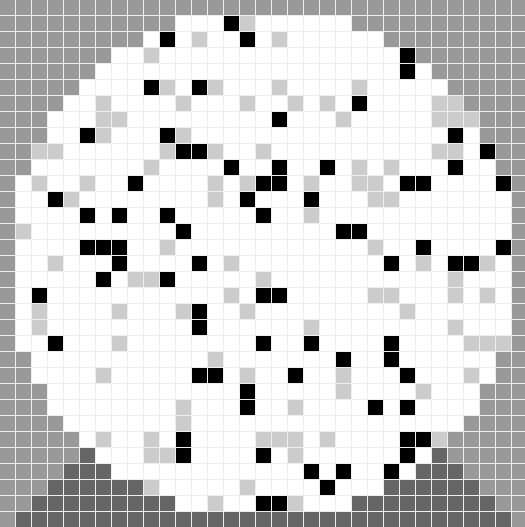
\includegraphics[width=84mm]{VS_Test_0001.png}
\caption{An initial cell-space configuration ($R = 16$, 
$\theta = 90^\circ$, $p_V = 9\%$, $p_S = 12\%$).  On the 
inside, black cells represent vesicles while the light grey 
cells are synapsins.  White cells are empty.  On the 
outside, the dark region at the bottom is the active zone, 
while the remainder are normal membrane cells.  Though it
is not part of the model, one could imagine a connection
to the axon of the neuron somewhere near the top. }
\label{fig:Initial}
\end{figure}
\\

\subsection{Transitions} \label{Transitions}
Used as an argument in transition functions, the state function $s$ 
gives the cell state for each cell in a neighborhood.  The expression
$s([1, 0])$, for example, represents the state of the cell with 
coordinates [1, 0] relative to the cell in question.
\begin{displaymath} \begin{array}{l}
s([i, j]) \in S; \\
\\
\hspace{16pt} [i, j] \in N
\end{array} \end{displaymath}
The functions $type$, $b$, $\Phi$, $\phi$, $v$, $z$, and $\sigma$ are
defined implicitly by the equation below.  It will be assumed that they 
are all available in whatever context the state function $s$ is 
available.  The expression $z([1, 0])$, for example, gives the priority
number of the cell with coordinates [1, 0] relative to the cell in 
question.
\begin{displaymath} \begin{array}{l}
s([i, j]) = [\\
\hspace{16pt} type([i, j]), \\
\hspace{16pt} b([i, j]), \\
\hspace{16pt} \Phi([i, j]), \\
\hspace{16pt} \phi([i, j]), \\
\hspace{16pt} v([i, j]), \\
\hspace{16pt} z([i, j]), \\
\hspace{16pt} \sigma([i, j])]
\end{array} \end{displaymath}
For convenience, the variables $type_0$, $b_0$, $\Phi_0$, $\phi_0$, 
$v_0$, $z_0$, and $\sigma_0$ will be used to represent the state of
the cell in question.  The expression $\Phi_0$, for example, will be 
used as an alternative to $\Phi([0, 0])$.
\begin{displaymath} \begin{array}{l}
s([0, 0]) = [type_0, b_0, \Phi_0, \phi_0, v_0, z_0, \sigma_0]
\end{array} \end{displaymath}
The time advance function $ta$ is defined as follows.
\begin{displaymath} \begin{array}{l}
ta(s) = \sigma_0
\end{array} \end{displaymath}
The local computing function $\tau$ is partially defined below.  The
eight phase-specific local computing functions ($\tau_{starting}$, 
$\tau_{holding}$, etc.) will be defined in subsequent subsections.
\begin{displaymath} \begin{array}{l}
\tau(s) = \left( \begin{array}{ll} \phi_0 = starting  & \rightarrow \tau_{starting}(s) \\
                                   \phi_0 = holding   & \rightarrow \tau_{holding}(s) \\
                                   \phi_0 = selecting & \rightarrow \tau_{selecting}(s) \\
                                   \phi_0 = binding_S & \rightarrow \tau_{binding_S}(s) \\
                                   \phi_0 = binding_V & \rightarrow \tau_{binding_V}(s) \\
                                   \phi_0 = aiming    & \rightarrow \tau_{aiming}(s) \\
                                   \phi_0 = steering  & \rightarrow \tau_{steering}(s) \\
                                   \phi_0 = moving    & \rightarrow \tau_{moving}(s) \end{array} \right)
\end{array} \end{displaymath}
Several functions are defined here for convenience.  The function
$any_{type}$ indicates whether any of the adjacent cells are of the
indicated type.
\begin{displaymath} \begin{array}{l}
any_{type}(s, type') = \\
\hspace{16pt} (type([1, 0]) = type') \vee (type([-1, 0]) = type') \vee \\
\hspace{16pt} (type([0, 1]) = type') \vee (type([0, -1]) = type') 
\end{array} \end{displaymath}
The function $any_{b_0}$ indicates whether the state function $b_0$ 
contains the indicated binding-related value.
\begin{displaymath} \begin{array}{l}
any_{b_0}(s, b_0') = \\
\hspace{16pt} (b_0([1, 0]) = b_0') \vee (b_0([-1, 0]) = b_0') \vee \\
\hspace{16pt} (b_0([0, 1]) = b_0') \vee (b_0([0, -1]) = b_0') 
\end{array} \end{displaymath}
If any of the adjacent cells have the indicated action state, $any_\Phi$
will yield a truthful result. 
\begin{displaymath} \begin{array}{l}
any_\Phi(s, \Phi') = \\
\hspace{16pt} (\Phi([1, 0]) = \Phi') \vee (\Phi([-1, 0]) = \Phi') \vee \\
\hspace{16pt} (\Phi([0, 1]) = \Phi') \vee (\Phi([0, -1]) = \Phi') 
\end{array} \end{displaymath}
If any of the adjacent cells have the indicated phase, $any_\phi$
will be true. 
\begin{displaymath} \begin{array}{l}
any_\phi(s, \phi') = \\
\hspace{16pt} (\phi([1, 0]) = \phi') \vee (\phi([-1, 0]) = \phi') \vee \\
\hspace{16pt} (\phi([0, 1]) = \phi') \vee (\phi([0, -1]) = \phi') 
\end{array} \end{displaymath}
The function $uniform$ results in a random value based on a uniform 
probability distribution.  The range lies between, but does include, 
0 and 1.
\begin{displaymath} \begin{array}{l}
uniform()
\end{array} \end{displaymath}
The expression below results in a value randomly selected from the 
vector $V$.  All values of $V$ are given an equal probability.
\begin{displaymath} \begin{array}{l}
random(V)
\end{array} \end{displaymath}



\subsection{Action Potentials}
Action potentials are triggered by events external to the Cell-DEVS
coupled modeled.  The input is received on the port $in$, which is 
directed to cell $[0, 0]$.  Any other membrane cell could have been 
used.
The receipt of an action potential changes the cell's action state,
as indicated by the equation below.  Also note the change in 
$\sigma$, the time remaining until the next internal event.
\begin{displaymath} \begin{array}{l}
\delta_{ext}(s, e, [in, \Phi']) = [type_0, b_0, \Phi_0', \phi_0, v_0, z_0, \sigma_0']; \\
\\
\hspace{16pt} \Phi_0' = \Phi' \\
\\
\hspace{16pt} \sigma_0' = \sigma_0 - e
\end{array} \end{displaymath}
Action-potential-related information is propagated in the $starting$ 
phase, and sustained during the $holding$ phase.  Because the 
$starting$ phase has instantaneous events, the conditional
formula below is necessary.  It states that if any of a
cell's adjacent neighbors is in the $holding$ phase, that cell must 
itself transition to the $holding$ phase without delay.  This need
to immediately update the phase is a recurring theme in the
model.
\begin{displaymath} \begin{array}{l}
\tau_{starting}(s) = \left( \begin{array}{ll} any_\phi(s, \phi_0')      & \rightarrow s_{now}' \\
                                              \neg any_\phi(s, \phi_0') & \rightarrow \tau_{starting}'(s) \end{array} \right); \\
\\
\hspace{16pt} \phi_0' = holding \\
\\
\hspace{16pt} s_{now}' = [type_0, b_0, \Phi_0, \phi_0', v_0, z_0, \sigma_0']; \\
\\
\hspace{16pt} \hspace{16pt} \sigma_0' = 0
\end{array} \end{displaymath}
If the cell is in a $holding_{[...]}$ action state, but at least one of its 
adjacent neighbors is $starting_{[...]}$, then the cell
adopts the new state without delay.  It also adopts the appropriate 
$starting_{[...]}$ value 
if the neighbor's value is $receiving_{[...]}$. Once
a cell's action state value changes, it then propagates this information to other
neighboring cells.\\
\\
A transition from $holding_{rest}$ to 
$starting_{act}$ indicates the beginning of an action potential.  The
transition from $holding_{act}$ to $starting_{rest}$ indicates that 
the chemical reactions induced by the action potential have subsided.
This simple "ON-or-OFF" model of action potentials suffices to break
up vesicle-synapsin clusters. \\
\\
The formulas below specify the propagation of action states.  If none
of a cell's neighbors are $starting$ a new action state, then the cell
transitions to the $holding$ phase in 1 time unit.  Note that this
delayed transition will be interrupted if a neighbor's state changes
within that time.
\begin{displaymath} \begin{array}{l}
\tau_{starting}'(s) = \left( \begin{array}{ll} any_{act}        & \rightarrow s_{act} \\
                                               any_{rest}       & \rightarrow s_{rest} \\
                                               \neg any_{start} & \rightarrow s_{later} \end{array} \right); \\
\\
\hspace{16pt} any_{act} = \\
\hspace{16pt} \hspace{16pt} ((\Phi_0 = holding_{act}) \wedge any_\Phi(s, starting_{act})) \vee \\
\hspace{16pt} \hspace{16pt} (\Phi_0 = receiving_{act}) \\
\\
\hspace{16pt} any_{rest} = \\
\hspace{16pt} \hspace{16pt} ((\Phi_0 = holding_{rest}) \wedge any_\Phi(s, starting_{rest})) \vee \\
\hspace{16pt} \hspace{16pt} (\Phi_0 = receiving_{rest}) \\
\\
\hspace{16pt} any_{starting} = any_{act} \vee any_{rest} \\
\\
\hspace{16pt} s_{act} = [type_0, b_0, \Phi_0', \phi_0, v_0, z_0, \sigma_0']; \\
\\
\hspace{16pt} \hspace{16pt} \Phi_0' = starting_{act} \\
\\
\hspace{16pt} \hspace{16pt} \sigma_0' = 0 \\
\\
\hspace{16pt} s_{rest} = [type_0, b_0, \Phi_0', \phi_0, v_0, z_0, \sigma_0']; \\
\\
\hspace{16pt} \hspace{16pt} \Phi_0' = starting_{rest} \\
\\
\hspace{16pt} \hspace{16pt} \sigma_0' = 0 \\
\\
\hspace{16pt} s_{later} = [type_0, b_0, \Phi_0, \phi_0', v_0, z_0, \sigma_0']; \\
\\
\hspace{16pt} \hspace{16pt} \phi_0' = holding \\
\\
\hspace{16pt} \hspace{16pt} \sigma_0' = 1 
\end{array} \end{displaymath}
Once a $starting_{[...]}$ action state has been propagated during the $starting$ 
phase, it must be converted to a corresponding $holding_{[...]}$ state during the
$holding$ phase. For example, suppose the presynaptic nerve terminal is at rest.  When an 
action potential arrives, the $\Phi_0$ of cell $[0,0]$ becomes $receiving_{act}$.
Sometime later, during the $starting$ phase, every cell becomes $starting_{act}$.  
After 1 time unit, during the $holding$ phase, every cell becomes $holding_{act}$.
A similar process takes place when the cell-space returns to the rest state. \\
\\
As indicated below, a cell in the $holding$ phase enters the $selecting$ phase
if any of its adjacent neighbors is in the $selecting$ phase.  The 
$B_{selecting}$ function will be explained in section \ref{Binding}.
\begin{displaymath} \begin{array}{l}
\tau_{holding}(s) = \left( \begin{array}{ll} any_\phi(s, \phi_0')      & \rightarrow s_{now} \\
                                             \neg any_\phi(s, \phi_0') & \rightarrow \tau_{holding}'(s) \end{array} \right); \\
\\
\hspace{16pt} \phi_0' = selecting \\
\\
\hspace{16pt} s_{now} = [type_0, b_0', \Phi_0, \phi_0', v_0, z_0, \sigma_0']; \\
\\
\hspace{16pt} \hspace{16pt} b_0' = B_{selecting}(s) \\
\\
\hspace{16pt} \hspace{16pt} \sigma_0' = 0
\end{array} \end{displaymath}
The formulas below convert $starting_{[...]}$ action states into corresponding 
$holding_{[...]}$ action states.  
\begin{displaymath} \begin{array}{l}
\tau_{holding}'(s) = \left( \begin{array}{ll} is_{starting_{act}}  & \rightarrow s_{act} \\
                                              is_{starting_{rest}} & \rightarrow s_{rest} \\
                                              \neg is_{starting}   & \rightarrow s_{later} \end{array} \right); \\
\\
\hspace{16pt} is_{starting_{act}} = (\Phi_0 = starting_{act}) \\
\\
\hspace{16pt} is_{starting_{rest}} = (\Phi_0 = starting_{rest}) \\
\\
\hspace{16pt} is_{starting} = is_{starting_{act}} \vee is_{starting_{rest}} \\
\\
\hspace{16pt} s_{act} = [type_0, b_0, \Phi_0', \phi_0, v_0, z_0, \sigma_0']; \\
\\
\hspace{16pt} \hspace{16pt} \Phi_0' = holding_{act} \\
\\
\hspace{16pt} \hspace{16pt} \sigma_0' = 0 \\
\\
\hspace{16pt} s_{rest} = [type_0, b_0, \Phi_0', \phi_0, v_0, z_0, \sigma_0']; \\
\\
\hspace{16pt} \hspace{16pt} \Phi_0' = holding_{rest} \\
\\
\hspace{16pt} \hspace{16pt} \sigma_0' = 0 \\
\\
\hspace{16pt} s_{later} = [type_0, b_0', \Phi_0, \phi_0', v_0, z_0, \sigma_0']; \\
\\
\hspace{16pt} \hspace{16pt} b_0' = B_{selecting}(s) \\
\\
\hspace{16pt} \hspace{16pt} \phi_0' = selecting \\
\\
\hspace{16pt} \hspace{16pt} \sigma_0' = 1 
\end{array} \end{displaymath}
If, or when, there are no $starting_{[...]}$ values to convert, a delay of 1 
time unit elapses and the cell enters the $selecting$ phase.  This is the 
first step in the vesicle-synapsin binding process.

\subsection{Vesicle-Synapsin Binding} \label{Binding}
After handling information related to action potentials, but before
vesicles and synapsins move, vesicle-synapsin bindings are permitted 
to change.  Adjacent but unbound vesicle and synapsins may bind 
together, while those that are already bound may separate. \\
\\
When a cell enters the $selecting$ phase, its $b_0$ function
is replaced with the result of the $B_{selecting}$ function.
The $b_0$ value is only changed if the cell is either a synapsin
or a vesicle.  If it is a synapsin, then the result of $b_0$ 
becomes $free$ in any direction that does not point to an
adjacent vesicle.  If it does point to a vesicle, $b_S'$ must
be evaluated.  For vesicles, $b_0$ results in $looking$ for each
direction that points to an adjacent synapsin.  Otherwise, the
result is $free$.
\begin{displaymath} \begin{array}{l}
B_{selecting}(s) = \left( \begin{array}{ll} type_0 = synapsin  & \rightarrow b_S \\
                                            type_0 = vesicle   & \rightarrow b_V \\
                                            \neg is_{particle} & \rightarrow b_0 \end{array} \right); \\
\\
\hspace{16pt} is_{particle} = type_0 \in \{ vesicle, synapsin\} \\
\\
\hspace{16pt} b_S([i, j]) = \\
\hspace{16pt} \hspace{16pt} \left( \begin{array}{ll} type([i, j]) \ne vesicle & \rightarrow free \\
                                                     type([i, j]) = vesicle   & \rightarrow b_S'(s, [i, j]) \end{array} \right) \\
\\
\hspace{16pt} b_V([i, j]) = \\
\hspace{16pt} \hspace{16pt} \left( \begin{array}{ll} type([i, j]) \ne synapsin & \rightarrow free \\
                                                     type([i, j]) = synapsin   & \rightarrow looking \end{array} \right)
\end{array} \end{displaymath}
In the case of a synapsin with a adjacent vesicle, the corresponding
result of $b_0$ depends first on whether the pair are already
bound.  If so, the result becomes $unseeking$, which can be
interpreted as "seeking separation".  If the pair are not already
bound, then the $b_{free}$ function is evaluated.
\begin{displaymath} \begin{array}{l}
b_S'(s, [i, j]) = \\
\hspace{16pt} \left( \begin{array}{ll} b_0([i, j]) = binding & \rightarrow unseeking \\
                                       b_0([i, j]) = free    & \rightarrow b_{free}(s, [i, j]) \end{array} \right)
\end{array} \end{displaymath}
Complications arise from the fact that a synapsin can only bind
in two opposite directions.  If the synapsin is binding the 
direction $[-i, -j]$, then it may seek a vesicle in direction $[i, j]$.
In this case, $b_0([i, j])$ becomes $seeking$.  Otherwise,
$b_{free}'$ is evaluated.
\begin{displaymath} \begin{array}{l}
b_{free}(s, [i, j]) = \\
\hspace{16pt} \left( \begin{array}{ll} b_0([-i, -j]) = binding & \rightarrow seeking \\
                                       b_0([-i, -j]) = free    & \rightarrow b_{free}'(s, [i, j]) \end{array} \right)
\end{array} \end{displaymath}
In the case that the synapsin is not binding in the direction opposite 
$[i, j]$, the two perpendicular directions are checked.  If the
synapsin is binding in either of these directions, its alignment
prohibits binding in the direction $[i, j]$.  The result of 
$b_0([i, j])$ therefore becomes $free$.  Otherwise,
$b_{free}''$ is evaluated.
\begin{displaymath} \begin{array}{l}
b_{free}'(s, [i, j]) = \\
\hspace{16pt} \left( \begin{array}{ll} binding_{perp}      & \rightarrow free \\
                                       \neg binding_{perp} & \rightarrow b_{free}''(s, [i, j]) \end{array} \right); \\
\\
\hspace{16pt} binding_{perp} = \\
\hspace{16pt} \hspace{16pt} (b_0([j, i]) = binding) \vee (b_0([-j, -i]) = binding)
\end{array} \end{displaymath}
In the final case, the synapsin is not binding in any direction.  
If then has a 50\% chance of $seeking$ the vesicle at $[i, j]$ as
a candidate for binding.
\begin{displaymath} \begin{array}{l}
b_{free}''(s, [i, j]) = \\
\hspace{16pt} \left( \begin{array}{ll} is_{aligned} & \rightarrow seeking \\
                                       \neg is_{aligned} & \rightarrow free \end{array} \right); \\
\\
\hspace{16pt} is_{aligned} = \\
\hspace{16pt} \hspace{16pt} ((|i| = 1) \wedge is_{vertical}) \vee ((|j| = 1) \wedge \neg is_{vertical})
\end{array} \end{displaymath}
Note that the random value of $is_{vertical}$ is evaluated once 
per cell, not once per direction. 
\begin{displaymath} \begin{array}{l}
is_{vertical} = uniform() < 0.5
\end{array} \end{displaymath}
The complex $B_{selecting}$ function is evaluated during the transition
into the $selecting$ phase.  Once this phase begins, its sole purpose
is to waste 1 time unit to ensure that $B_{selecting}$ has been 
evaluated on each cell.
\begin{displaymath} \begin{array}{l}
\tau_{selecting}(s) = [type_0, b_0, \Phi_0, \phi_0', v_0, z_0, \sigma_0']; \\
\\
\hspace{16pt} \phi_0' = binding_S \\
\\
\hspace{16pt} \sigma_0' = 1
\end{array} \end{displaymath}
The $binding_S$ phase is when the synapsins firmly decide whether
they will bind with adjacent vesicles.  It is followed by the 
$binding_V$ phase, in which vesicles identify bindings by looking
at the synapsins.  The formula below indicates an immediate 
transition to the $binding_V$ phase in the event that any of a cell's
adjacent neighbors is already in that phase.  Otherwise, 
$\tau_{binding_S}'$ is evaluated.
\begin{displaymath} \begin{array}{l}
\tau_{binding_S}(s) = \left( \begin{array}{ll} any_\phi(s, \phi_0')      & \rightarrow s_{now} \\
                                               \neg any_\phi(s, \phi_0') & \rightarrow \tau_{binding_S}'(s) \end{array} \right); \\
\\
\hspace{16pt} \phi_0' = binding_V \\
\\
\hspace{16pt} s_{now} = [type_0, b_0, \Phi_0, \phi_0', v_0, z_0, \sigma_0']; \\
\\
\hspace{16pt} \hspace{16pt} \sigma_0' = 0 
\end{array} \end{displaymath}
An unresolved direction, in the case of a synapsin, is one
for which the $b_0$ function results in $seeking$ or
$unseeking$.  If there are any unresolved directions,
$\tau_{binding_S}''$ is evaluated.
\begin{displaymath} \begin{array}{l}
\tau_{binding_S}'(s) = \left( \begin{array}{ll} any_{unresolved}      & \rightarrow \tau_{binding_S}''(s) \\
                                                \neg any_{unresolved} & \rightarrow s_{later}' \end{array} \right); \\
\\
\hspace{16pt} any_{unresolved} = \\
\hspace{16pt} \hspace{16pt} any_{b_0}(s, seeking) \vee any_{b_0}(s, unseeking) \\
\\
\hspace{16pt} s_{later}' = [type_0, b_0, \Phi_0, \phi_0', v_0, z_0, \sigma_0']; \\
\\
\hspace{16pt} \hspace{16pt} \phi_0' = binding_V \\
\\
\hspace{16pt} \hspace{16pt} \sigma_0' = 1 
\end{array} \end{displaymath}
When $\tau_{binding_S}''$ is evaluated, $b_0$ is changed 
in each unresolved direction.  If it results in $seeking$ for one
direction, there is a probability $p$ that it will become
$binding$.  Otherwise it will become $free$.  If $b_0$ results
in $unseeking$ for a direction, there is a probability $q$ 
that it will become $free$.  Otherwise, it becomes $binding$.
Here $p$ and $q$ depend on the action state.  If the 
presynaptic nerve terminal is at rest, the model parameters 
$p_{rest}$ and $q_{rest}$ are used.  If the terminal is
responding to an action potential, then $p_{act}$ and $q_{act}$ 
are used.
\begin{displaymath} \begin{array}{l}
\tau_{binding_S}''(s) = [type_0, b_0', \Phi_0, \phi_0, v_0, z_0, \sigma_0']; \\
\\
\hspace{16pt} b_0'([i, j]) = \left( \begin{array}{ll} b_0([i, j]) = seeking   & \rightarrow b_p([i, j]) \\
                                                      b_0([i, j]) = unseeking & \rightarrow b_q([i, j]) \\
                                                      resolved                & \rightarrow b_0([i, j]) \end{array} \right); \\
\\
\hspace{16pt} \hspace{16pt} resolved = \\
\hspace{16pt} \hspace{16pt} \hspace{16pt} (b_0([i, j]) \ne seeking) \wedge \\
\hspace{16pt} \hspace{16pt} \hspace{16pt} (b_0([i, j]) \ne unseeking) \\
\\
\hspace{16pt} b_p([i, j]) = \left( \begin{array}{ll} rand < p   & \rightarrow binding \\
                                                     rand \ge p & \rightarrow free \end{array} \right); \\
\\
\hspace{16pt} \hspace{16pt} p = \left( \begin{array}{ll} \Phi_0 = holding_{rest} & \rightarrow p_{rest} \\
                                                         \Phi_0 = holding_{act}  & \rightarrow p_{act} \end{array} \right) \\
\\
\hspace{16pt} \hspace{16pt} rand = uniform() \\
\\
\hspace{16pt} b_q([i, j]) = \left( \begin{array}{ll} rand < q   & \rightarrow free \\
                                                     rand \ge q & \rightarrow binding \end{array} \right); \\
\\
\hspace{16pt} \hspace{16pt} q = \left( \begin{array}{ll} \Phi_0 = holding_{rest} & \rightarrow q_{rest} \\
                                                         \Phi_0 = holding_{act}  & \rightarrow q_{act} \end{array} \right) \\
\\
\hspace{16pt} \hspace{16pt} rand = uniform() \\
\\
\hspace{16pt} \sigma_0' = 0 \\
\end{array} \end{displaymath}
Once synapsins have chosen their binding directions, and
the cell-space transitions from $binding_S$ to $binding_V$,
the vesicles respond.  The first thing specified is the 
condition where a cell's neighbor has already transitioned
to the $aiming$ phase, in which case that cell must also
transition.  Otherwise $\tau_{binding_V}'$ is evaluated.
The functions $V_{aiming}$ and $Z_{aiming}$ are explained 
in section \ref{Motion}.
\begin{displaymath} \begin{array}{l}
\tau_{binding_V}(s) = \left( \begin{array}{ll} any_\phi(s, \phi_0')      & \rightarrow s_{now} \\
                                               \neg any_\phi(s, \phi_0') & \rightarrow \tau_{binding_V}'(s) \end{array} \right); \\
\\
\hspace{16pt} \phi_0' = aiming \\
\\
\hspace{16pt} s_{now} = [type_0, b_0, \Phi_0, \phi_0', V_{aiming}(s), Z_{aiming}(s), \sigma_0']; \\
\\
\hspace{16pt} \hspace{16pt} \sigma_0' = 0 
\end{array} \end{displaymath}
In the case of a vesicle, an unresolved direction is one for
which $b_0$ results in $looking$.  The function $\tau_{binding_V}''$ 
is evaluated if any directions are unresolved.
\begin{displaymath} \begin{array}{l}
\tau_{binding_V}'(s) = \left( \begin{array}{ll} any_{unresolved}      & \rightarrow \tau_{binding_V}''(s) \\
                                                \neg any_{unresolved} & \rightarrow s_{later}' \end{array} \right); \\
\\
\hspace{16pt} any_{unresolved} =  any_{b_0}(s, looking) \\
\\
\hspace{16pt} s_{later}' = [type_0, b_0, \Phi_0, \phi_0', V_{aiming}(s), Z_{aiming}(s), \sigma_0']; \\
\\
\hspace{16pt} \hspace{16pt} \phi_0' = aiming \\
\\
\hspace{16pt} \hspace{16pt} \sigma_0' = 1 
\end{array} \end{displaymath}
When $\tau_{binding_V}''$ is evaluated, the result is a change in 
$b_0([i, j])$ for each unresolved direction $[i, j]$.  Suppose the 
adjacent synapsin, in direction $[i. j]$, is binding in the opposite 
direction, $[-i, -j]$.  In that case, $b_0([i, j])$ is $binding$.
Otherwise it is $free$.
\begin{displaymath} \begin{array}{l}
\tau_{binding_V}''(s) = [type_0, b_0', \Phi_0, \phi_0, v_0, z_0, \sigma_0']; \\
\\
\hspace{16pt} b_0'([i, j]) = \left( \begin{array}{ll} b_0([i, j]) = looking   & \rightarrow b_0''([i, j]) \\
                                                      b_0([i, j]) \ne looking & \rightarrow b_0([i, j]) \end{array} \right) \\
\\
\hspace{16pt} b_0''([i, j]) = \\
\hspace{16pt} \hspace{16pt} \left( \begin{array}{ll} b_{adj}([-i, -j]) = binding & \rightarrow binding \\
                                                     b_{adj}([-i, -j]) = free    & \rightarrow free \end{array} \right); \\
\\
\hspace{16pt} \hspace{16pt} b_{adj} = b([i, j]) \\
\\
\hspace{16pt} \sigma_0' = 0 \\
\end{array} \end{displaymath}
By the time the cell-space transitions into the $aiming$ phase, 
all bindings between vesicles and synapsins have been resolved.

\subsection{Cluster Motion} \label{Motion}
While it would be relatively straightforward to allow 
isolated single-cell particles to move randomly through 
the presynaptic nerve terminal, it is challenging to 
specify the motion of vesicle-synapsin clusters.  A 
cluster is any group of vesicles and synapsins connected
through $binding$ links defined by the $b_0$ functions. 
Clusters move randomly, remaining intact and avoiding
obstacles such as other clusters.  The algorithm designed
to accomplish this is based on priority numbers. \\
\\
Upon transitioning to the $aiming$ phase, the intended 
direction $v_0$ and priority number $z_0$ of each cell 
may be changed.  The new values are obtained from the 
$V_{aiming}$ and $Z_{aiming}$ functions respectively.
If a cell is a vesicle or synapsin, and if it is not
adjacent to the active zone, then both the direction
and priority number are randomized.  Otherwise the
direction is $[0,0]$, indicating no motion.  In this
case, the priority number given to empty cells is 1, 
which is the weakest number.  If the motionless cell
is not empty, the priority number is zero, which is
the strongest.
\begin{displaymath} \begin{array}{l}
V_{aiming}(s) = \left( \begin{array}{ll} is_{movable}(s)      & \rightarrow V_{random}() \\
                                         \neg is_{movable}(s) & \rightarrow [0, 0]  \end{array} \right) \\
\\
Z_{aiming}(s) = \left( \begin{array}{ll} is_{movable}(s)      & \rightarrow Z_{random}() \\
                                         \neg is_{movable}(s) & \rightarrow Z_{frozen}(s) \end{array} \right) \\
\\
is_{movable}(s) = \\
\hspace{16pt} (type_0 \in \{ vesicle, synapsin\}) \wedge \\
\hspace{16pt} \neg any_{type}(s, zone) \\
\\
V_{random}() = random([[1, 0], [0, 1], [-1, 0], [0, -1]]) \\
\\
Z_{random}() = uniform() \\
\\
Z_{frozen}(s) = \left( \begin{array}{ll} type_0 = empty   & \rightarrow 1 \\
                                          type_0 \ne empty & \rightarrow 0 \end{array} \right) \\
\end{array} \end{displaymath}
The first phase associated with cluster motion is
$aiming$.  A cell, with any neighbors
that have already advanced to the $steering$ phase,
must itself advance.
\begin{displaymath} \begin{array}{l}
\tau_{aiming}(s) = \left( \begin{array}{ll} any_\phi(s, \phi_0')      & \rightarrow s_{now}' \\
                                            \neg any_\phi(s, \phi_0') & \rightarrow \tau_{aiming}'(s) \end{array} \right); \\
\\
\hspace{16pt} \phi_0' = steering \\
\\
\hspace{16pt} s_{now}' = [type_0, b_0, \Phi_0, \phi_0', v_0, z_0, \sigma_0']; \\
\\
\hspace{16pt} \hspace{16pt} \sigma_0' = 0
\end{array} \end{displaymath}
During the $aiming$ phase, directions and priority numbers 
are repeatedly shared within each cluster.  A cell will 
adopt these values from an adjacent neighbor, provided that
the neighbor has a lower priority number than that of the
cell itself.  The process ends when each vesicle and 
synapsin has the same direction and priority number as any 
other component in the same cluster.  \\
\\
It is useful to define a function $g_{aiming}$, which results 
in a truthful value if a neighbor at $[i, j]$ has a lower
priority number and is bound to the cell.  Another function,
$G_{aiming}$, is truthful if all neighbors have advanced past
the $binding_V$ phase, and $g_{aiming}([i, j])$ is true for
any $[i, j]$ describing an adjacent cell.
\begin{displaymath} \begin{array}{l}
g_{aiming}(s, [i, j]) = (z([i, j]) < z_0) \wedge (s_0([i, j]) = binding) \\
\\
G_{aiming}(s) = \neg any_{\phi}(s, binding_V) \wedge ( \\
\hspace{16pt} g_{aiming}(s, [1, 0]) \vee g_{aiming}(s, [-1, 0]) \vee \\
\hspace{16pt} g_{aiming}(s, [0, 1]) \vee g_{aiming}(s, [0, -1]))
\end{array} \end{displaymath}
So long as the result of $G_{aiming}$ is false, there is
nothing to do other than transition to the $steering$ phase
after 1 time unit.
\begin{displaymath} \begin{array}{l}
\tau_{aiming}'(s) = \left( \begin{array}{ll} G_{aiming}(s)      & \rightarrow \tau_{aiming}''(s) \\
                                             \neg G_{aiming}(s) & \rightarrow s_{later}' \end{array} \right); \\
\\
\hspace{16pt} s_{later}' = [type_0, b_0, \Phi_0, \phi_0', v_0, z_0, \sigma_0']; \\
\\
\hspace{16pt} \hspace{16pt} \phi_0' = steering \\
\\
\hspace{16pt} \hspace{16pt} \sigma_0' = 1 
\end{array} \end{displaymath}
If $G_{aiming}$ is true, the lower priority number and 
direction are copied from the adjacent neighbor.
\begin{displaymath} \begin{array}{l}
\tau_{aiming}''(s) = \left( \begin{array}{ll} g_{aiming}(s, [1, 0]) & \rightarrow obey(s, [1, 0]) \\
                                              g_{aiming}(s, [0, 1]) & \rightarrow obey(s, [0, 1]) \\
                                              g_{aiming}(s, [-1, 0]) & \rightarrow obey(s, [-1, 0]) \\
                                              g_{aiming}(s, [0, -1]) & \rightarrow obey(s, [0, -1]) \end{array} \right) \\
\end{array} \end{displaymath}
The copying is specified by the $obey$ function below.
\begin{displaymath} \begin{array}{l}
obey(s, [i, j]) = [type_0, b_0, \Phi_0, \phi_0, v_0', z_0', \sigma_0']; \\
\\
\hspace{16pt} v_0' = v([i, j]) \\
\\
\hspace{16pt} z_0' = z([i, j]) \\
\\
\hspace{16pt} \sigma_0' = 0
\end{array} \end{displaymath}
By the time the cell-space transitions beyond the $aiming$ phase, 
all particles and clusters have an intended direction.
That direction may change, however.  Vesicles and synapsins 
must not collide, and must not enter the membrane.  All
possible collisions are to be resolved during the $steering$
phase. \\
\\
First, cells are to transition to the $moving$ phase if 
adjacent neighbors have already done so.  
\begin{displaymath} \begin{array}{l}
\tau_{steering}(s) = \left( \begin{array}{ll} any_\phi(s, \phi_0')      & \rightarrow s_{now}' \\
                                              \neg any_\phi(s, \phi_0') & \rightarrow \tau_{steering}'(s) \end{array} \right); \\
\\
\hspace{16pt} \phi_0' = moving \\
\\
\hspace{16pt} s_{now}' = [type_0, b_0, \Phi_0, \phi_0', v_0, z_0, \sigma_0']; \\
\\
\hspace{16pt} \hspace{16pt} \sigma_0' = 0
\end{array} \end{displaymath}
As was the case in the $aiming$ phase, a direction and
priority number are copied from an adjacent cell only if
the priority number is lower.  In the case of $steering$,
any one of three conditions must also be met.  One of 
those case is the same as in the case of $aiming$; 
specifically, that the cell is bound to the adjacent 
neighbor.  Clearly, the two particles must have the
same direction. \\
\\
The second possible condition is that the cell is either
a vesicle or a synapsin, and is currently intending to 
move towards the adjacent neighbor with the lower priority
number.  This condition helps to prevent collisions. \\
\\
The third possible condition is that the adjacent neighbor
is a vesicle or synapsin, and the adjacent neighbor is 
intending to move towards the cell.  This also helps to 
prevent collisions.  Note that in this case, the cell in 
question may be empty.  In the $steering$ phase, empty 
cells can adopt directions from vesicles and synapsins. \\
\\
The conditions described above are defined formally in 
the function $g_{steering}$.
\begin{displaymath} \begin{array}{l}
g_{steering}(s, [i, j]) = \\
\hspace{16pt} (z([i, j]) < z_0) \wedge (\\
\hspace{16pt} \hspace{16pt} (s_0([i, j]) = binding) \vee \\
\hspace{16pt} \hspace{16pt} ((type_0 \in \{ vesicle, synapsin\}) \wedge \\
\hspace{16pt} \hspace{16pt} \hspace{16pt} (v_0 = [i, j])) \vee \\
\hspace{16pt} \hspace{16pt} ((type([i, j]) \in \{ vesicle, synapsin\}) \wedge \\
\hspace{16pt} \hspace{16pt} \hspace{16pt} (v([i, j]) = [-i, -j])))
\end{array} \end{displaymath}
Suppose that an empty cell has an approaching vesicle on 
either side.  Suppose also that the one on the right has 
a lower priority number.  The empty cell in the middle will
adopt the direction and priority number from the right.  In
this case, the direction is pointing to the left.  The 
vesicle on the left will then adopt this lower priority 
number as well, and reverse its direction.  This example
illustrates how a possible collision is avoided. \\
\\
Continuing the example above, suppose that the vesicle
on the right in now pushed upwards by a synapsin with a 
lower priority number.  The empty cell now has no 
approaching particles.  In order to reset its direction
and priority number, this condition checked using the 
function $\gamma_{steering}$.
\begin{displaymath} \begin{array}{l}
\gamma_{steering}(s, [i, j]) = \\
\hspace{16pt} (type_0 = empty) \wedge \\
\hspace{16pt} (v_0 = [i, j]) \wedge \\
\hspace{16pt} (v([i, j]) \ne [-i, -j])
\end{array} \end{displaymath}
All the conditions described above are combined into 
the single function $G_{steering}$.
\begin{displaymath} \begin{array}{l}
G_{steering}(s) = \neg any_{\phi}(s, aiming) \wedge ( \\
\hspace{16pt} g_{steering}(s, [1, 0]) \vee g_{steering}(s, [-1, 0]) \vee \\
\hspace{16pt} g_{steering}(s, [0, 1]) \vee g_{steering}(s, [0, -1]) \vee \\
\hspace{16pt} \gamma_{steering}(s, [1, 0]) \vee \gamma_{steering}(s, [-1, 0]) \vee \\
\hspace{16pt} \gamma_{steering}(s, [0, 1]) \vee \gamma_{steering}(s, [0, -1]))
\end{array} \end{displaymath}
As long as $G_{steering}(s)$ is false, a cell has nothing
to do except wait 1 time unit then transition to the 
$moving$ phase.
\begin{displaymath} \begin{array}{l}
\tau_{steering}'(s) = \left( \begin{array}{ll} G_{steering}(s)      & \rightarrow \tau_{steering}''(s) \\
                                               \neg G_{steering}(s) & \rightarrow s_{later}' \end{array} \right); \\
\\
\hspace{16pt} s_{later}' = [type_0, b_0, \Phi_0, \phi_0', v_0, z_0, \sigma_0']; \\
\\
\hspace{16pt} \hspace{16pt} \phi_0' = moving \\
\\
\hspace{16pt} \hspace{16pt} \sigma_0' = 1 
\end{array} \end{displaymath}
If $G_{steering}(s)$ is true, then one of the conditions 
that requires a change of direction and priority is also
true.  These possible changes are specified below.  The 
function $obey$ is the same as in the $aiming$ phase,
while $obey_{all}$ resets empty cells.
\begin{displaymath} \begin{array}{l}
\tau_{steering}''(s) = \\
\hspace{16pt} \left( \begin{array}{ll} g_{steering}(s, [1, 0]) & \rightarrow obey(s, [1, 0]) \\
                                       g_{steering}(s, [0, 1]) & \rightarrow obey(s, [0, 1]) \\
                                       g_{steering}(s, [-1, 0]) & \rightarrow obey(s, [-1, 0]) \\
                                       g_{steering}(s, [0, -1]) & \rightarrow obey(s, [0, -1]) \\
                                       \gamma_{steering}(s, [1, 0]) & \rightarrow obey_{all} \\
                                       \gamma_{steering}(s, [0, 1]) & \rightarrow obey_{all} \\
                                       \gamma_{steering}(s, [-1, 0]) & \rightarrow obey_{all} \\
                                       \gamma_{steering}(s, [0, -1]) & \rightarrow obey_{all} \end{array} \right); \\
\\
\hspace{16pt} obey_{all} = [type_0, b_0, \Phi_0, \phi_0, v_0', z_0', \sigma_0']; \\
\\
\hspace{16pt} \hspace{16pt} v_0' = [0, 0] \\
\\
\hspace{16pt} \hspace{16pt} z_0' = 1 \\
\\
\hspace{16pt} \hspace{16pt} \sigma_0' = 0
\end{array} \end{displaymath}
The final phase is $moving$.  At this point, all
vesicles and synapsins have intended directions.
These directions will not break bindings, and 
will not cause collisions.  The function
$g_{moving}$ indicates whether a cell has an 
incoming particle in a given direction.  The
function $G_{moving}$ indicates whether a cell
has an incoming particle in any direction.
\begin{displaymath} \begin{array}{l}
g_{moving}(s, [i, j]) = \\
\hspace{16pt} (type([i, j]) \in \{ vesicle, synapsin\}) \wedge \\
\hspace{16pt} (v([i, j]) = [-i, -j]) \\
\\
G_{moving}(s) = \\
\hspace{16pt} g_{moving}(s, [1, 0]) \vee g_{moving}(s, [-1, 0]) \vee \\
\hspace{16pt} g_{moving}(s, [0, 1]) \vee g_{moving}(s, [0, -1])
\end{array} \end{displaymath}
If a cell has an incoming particle, $\tau_{moving}'$ 
is evaluated.  Otherwise, its future state depends on
a function named $move$.
\begin{displaymath} \begin{array}{l}
\tau_{moving}(s) = \left( \begin{array}{ll} G_{moving}(s)      & \rightarrow \tau_{moving}'(s) \\
                                            \neg G_{moving}(s) & \rightarrow move(s) \end{array} \right)
\end{array} \end{displaymath}
The $\tau_{moving}'$ function obtains the $type_0$ 
and $b_0$ values from the cell with the incoming
vesicle or synapsin.  The transition occurs after 
1 time unit.
\begin{displaymath} \begin{array}{l}
\tau_{aiming}''(s) = \\
\hspace{16pt} \left( \begin{array}{ll} g_{moving}(s, [1, 0]) & \rightarrow from(s, [1, 0]) \\
                                       g_{moving}(s, [0, 1]) & \rightarrow from(s, [0, 1]) \\
                                       g_{moving}(s, [-1, 0]) & \rightarrow from(s, [-1, 0]) \\
                                       g_{moving}(s, [0, -1]) & \rightarrow from(s, [0, -1]) \end{array} \right); \\
\\
\hspace{16pt} from(s, [i, j]) = [type_0', b_0', \Phi_0, \phi_0', v_0', z_0', \sigma_0']; \\
\\
\hspace{16pt} \hspace{16pt} type_0' = type([i, j]) \\
\\
\hspace{16pt} \hspace{16pt} b_0' = b([i, j]) \\
\\
\hspace{16pt} \hspace{16pt} \phi_0' = starting \\
\\
\hspace{16pt} \hspace{16pt} v_0' = [0, 0] \\
\\
\hspace{16pt} \hspace{16pt} z_0' = 0 \\
\\
\hspace{16pt} \hspace{16pt} \sigma_0' = 1
\end{array} \end{displaymath}
If there are no incoming particles, the one
condition to check is whether the cell represents 
a vacating vesicle or synapsin.  If so, the
cell becomes empty.  Otherwise, its type 
remains as is.
\begin{displaymath} \begin{array}{l}
move(s) = \left( \begin{array}{ll} vacating      & \rightarrow from_{none} \\
                                   \neg vacating & \rightarrow s_{later}' \end{array} \right); \\
\\
\hspace{16pt} vacating = \\
\hspace{16pt} \hspace{16pt} (type([i, j]) \in \{ vesicle, synapsin\}) \wedge (v \ne [0, 0]) \\
\\
\hspace{16pt} from_{none} = [type_0', b_0', \Phi_0, \phi_0', v_0', z_0', \sigma_0']; \\
\\
\hspace{16pt} \hspace{16pt} type_0' = empty \\
\\
\hspace{16pt} \hspace{16pt} b_0'([i, j]) = free \\
\\
\hspace{16pt} \hspace{16pt} \phi_0' = starting \\
\\
\hspace{16pt} \hspace{16pt} v_0' = [0, 0] \\
\\
\hspace{16pt} \hspace{16pt} z_0' = 0 \\
\\
\hspace{16pt} \hspace{16pt} \sigma_0' = 1 \\
\\
\hspace{16pt} s_{later}' = [type_0, b_0, \Phi_0, \phi_0', v_0', z_0', \sigma_0']; \\
\\
\hspace{16pt} \hspace{16pt} \phi_0' = starting \\
\\
\hspace{16pt} \hspace{16pt} v_0' = [0, 0] \\
\\
\hspace{16pt} \hspace{16pt} z_0' = 0 \\
\\
\hspace{16pt} \hspace{16pt} \sigma_0' = 1 
\end{array} \end{displaymath}

\section{Implementation and Testing} \label{Implementation}
This sections discusses the implementation of 
the model, and presents the results of a selected test.  
\begin{figure*}[ht]
\centering
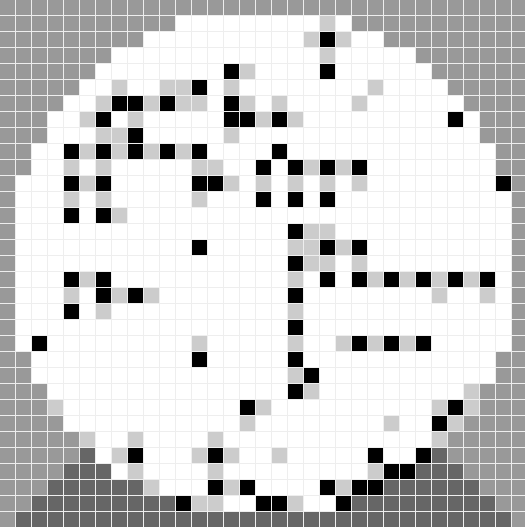
\includegraphics[width=56mm]{VS_Test_0600.png}
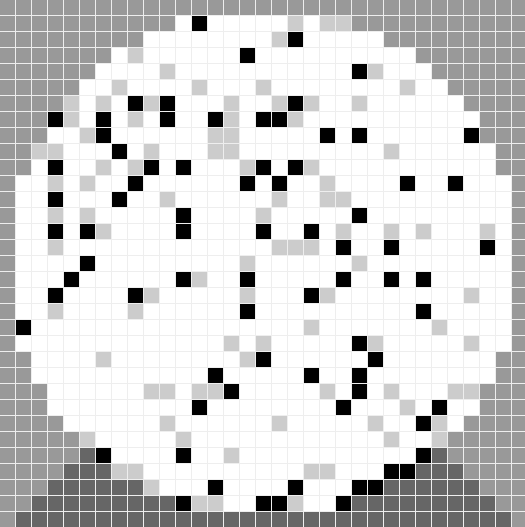
\includegraphics[width=56mm]{VS_Test_0641.png}
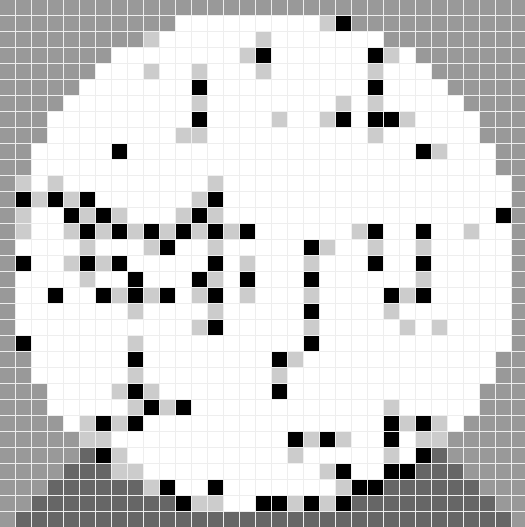
\includegraphics[width=56mm]{VS_Test_1240.png}
\caption{Three snapshots from the test described 
in the text.  The one on the left shows clusters 
formed after 75 cycles.  The first action potential 
arrived immediately after, and the resulting reaction
lasted 5 cycles.  Immediately after these 5 cycles, 
as shown in the center image, the vesicles and synapsins 
in the large clusters dispersed.  Different clusters
reformed, as shown on the right, after an additional 
75 cycles.  Black cells represent vesicles, while the 
light grey cells are synapsins. }
\label{fig:Results}
\end{figure*}

\subsection{CD++ Implementation}
The model was implemented using CD++.
This toolkit was developed in conjunction with a 
language designed specifically for the implementation
of Cell-DEVS models.  Macros were written to
separate the model parameters from the code, and
to facilitate the reuse of certain expressions.\\
\\
While the specification defines a single Cell-DEVS
coupled model, the implementation also included an
``axon'' model to provide external events at regular 
intervals.  The
axon model was given two parameters: one to represent
the number of cycles between action potentials, and
one to specify the duration of each reaction triggered
by an action potential.  A ``cycle'' is a complete
rotation through each of the eight phases, a time period
during which vesicles and synapsins can move at most 
once.  For convenience, the axon model was itself 
defined as a Cell-DEVS coupled model containing a 
single cell.  A DEVS atomic model could have been 
implemented instead. \\
\\
Extra conditions were added to the implementation to
address the possibility that two randomly-generated
priority numbers might be equal in value.  
Mathematically this is an impossibility, so the
specification is not incorrect for neglecting the
issue.  In the code, in
the event that conflicting directions and priority 
numbers are encountered, a vesicle or synapsin is
rendered motionless with a priority number of zero.

\subsection{Test Results}
Tests demonstrated that the model captures the desired
qualitative behaviour of vesicles and synapsins.  One 
such test involved the simulation of a cell-space with 
the following initial conditions.
\begin{displaymath} \begin{array}{l}
R = 8 \\
\\
\theta = 90^\circ \\
\\
p_V = 9\% \\
\\
p_S = 12\% 
\end{array} \end{displaymath}
In the model, vesicles and synapsins were given a
100\% chance of binding while the terminal was at
rest.  The probability of adjacent vesicles and 
synapsins binding was actually closer to 50\%, as
synapsins bind in only two of four directions.  A
1\% probability of separation was added to discourage 
the formation of extremely long and narrow clusters.
During an action-potential-induced reaction, the binding
probability was lowered to 10\%, while the probability 
of separation was raised to 50\%.
\begin{displaymath} \begin{array}{l}
p_{rest} = 100\% \\
\\
q_{rest} = 1\% \\
\\
p_{act} = 10\% \\
\\
q_{rest} = 50\%
\end{array} \end{displaymath}
At the beginning of the simulation, vesicles and 
synapsins were randomly distributed in the 
terminal.  Although this initial condition does
not represent reality, clusters began forming 
within the first few cycles.  As intended, the clusters mostly
broke up after the arrival of an action 
potential, but regrouped thereafter.\\
\\
Figure \ref{fig:Results} shows three 
snapshots from the simulation: one immediately
before the first action potential, the next 
immediately following the resulting reaction, and the
third immediately prior to the second action 
potential.  One can also observe vesicles and
synapsins in the vicinity of the active zone at
the bottom.  \\
\\
Clusters are smaller and more numerous
than they appear in the snapshots.  Noting that
synapsins may bind to at most two vesicles, one
can identify groups of adjacent, small clusters that
at first appear as single, large clusters.  The
tendency for clusters to form in straight lines was
not intended, but is a logical consequence of the
binding rules.  A greater value of $q$ would likely
result in rounder clusters, as the linear clusters
would be rendered unstable.

\section{Conclusions}
Simulations demonstrated that the model captured
the desired qualitative behaviour of vesicles 
and synapsins in presynaptic nerve terminals.
Specifically, test results showed the formation 
and break-up of clusters in response to action
potentials, the random motion of clusters, and
the docking of vesicles and synapsins near the
active zone.  No efforts have yet been made to 
assess the validity of the model, nor to optimize
the models parameters.\\
\\
The Cell-DEVS formalism proved particularly 
useful for the propagation of action-potential-related
information, and for the avoidance of 
collisions during cluster motion.  These aspects
of the model relied on instantaneous transitions.
In retrospect, the specification may
have been simpler if the zero-delay transitions
used for binding had been avoided. \\
\\
The cluster motion algorithm is the most 
interesting and perhaps the most novel aspect of
the model.  Unfortunately, it has two drawbacks:
inefficiency and asymmetry.  It is inefficient
because many random directions and priority numbers
are propagated, most of which are to be replaced 
with other directions and smaller priority numbers.
The motion of clusters is asymmetric because, in the
$steering$ phase, the final combination of 
directions depends on the order in which simultaneous
events are resolved.  If the order of events was 
itself randomized, there would be no bias.  But as
the order of events depends on positions and directions,
clusters will likely have a tendency to favour certain
directions over others.  The effect of this bias was
neither studied nor observed. \\
\\
Possible future enhancements include the adaptation of the
model to a 3-dimensional cell-space, and the fusion and 
formation of vesicles on the membrane.  It may also be
possible to change the vesicle-synapsin binding rules 
to better reflect reality.  One drawback of the Cell-DEVS 
approach is that it would be difficult to allow a cluster to rotate.
Representing long actin structures, which are known to influence 
vesicle-synapsin clusters, would also be a challenge. 

\bibliographystyle{ieeetr}
\bibliography{VS_Paper_2007-12}

\balancecolumns

\end{document}
